\documentclass[review]{elsarticle}

\usepackage{lineno,hyperref}
\modulolinenumbers[5]
\usepackage{amsmath}
\usepackage{lineno,hyperref}
\usepackage{siunitx}
\usepackage{csquotes}
\usepackage[table]{xcolor}
\usepackage{slashbox,booktabs}
\usepackage{color}
\usepackage{setspace}
\journal{Journal of \LaTeX\ Templates}

%%%%%%%%%%%%%%%%%%%%%%%
%% Elsevier bibliography styles
%%%%%%%%%%%%%%%%%%%%%%%
%% To change the style, put a % in front of the second line of the current style and
%% remove the % from the second line of the style you would like to use.
%%%%%%%%%%%%%%%%%%%%%%%

%% Numbered
%\bibliographystyle{model1-num-names}

%% Numbered without titles
%\bibliographystyle{model1a-num-names}

%% Harvard
%\bibliographystyle{model2-names.bst}\biboptions{authoryear}

%% Vancouver numbered
%\usepackage{numcompress}\bibliographystyle{model3-num-names}

%% Vancouver name/year
%\usepackage{numcompress}\bibliographystyle{model4-names}\biboptions{authoryear}

%% APA style
%\bibliographystyle{model5-names}\biboptions{authoryear}

%% AMA style
%\usepackage{numcompress}\bibliographystyle{model6-num-names}

%% `Elsevier LaTeX' style
\bibliographystyle{elsarticle-num}
%%%%%%%%%%%%%%%%%%%%%%%

\begin{document}
In the article contains eight figures, the eight figures are preseted in the following: 
\vspace{1 cm}
\begin{figure}[h]
	\centering
	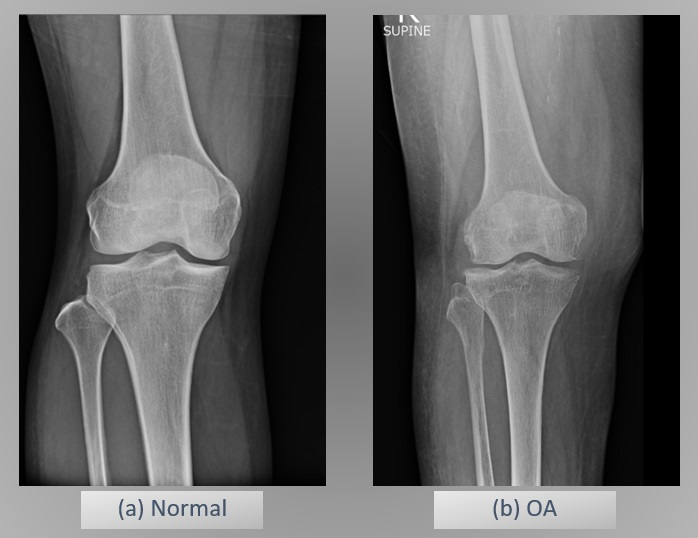
\includegraphics[width=0.7\linewidth]{pic/picOA}
	\caption{Normal and Osteoarthritis (OA) Knee X-ray Imagery.}
	\label{fig:picoa}
\end{figure}
\vspace{1 cm}
\begin{figure}[h!]
	\centering
	%%\includegraphics[width=0.99\linewidth]{./pic/fig1.png}	
	\includegraphics[width=0.99\linewidth]{./pic/fig1}
	\caption{Texture Analysis on Knee OA Classification Techniques.}
	\label{fig:framework}
\end{figure}
\vspace{1 cm}
\begin{figure}[h]
	\centering
	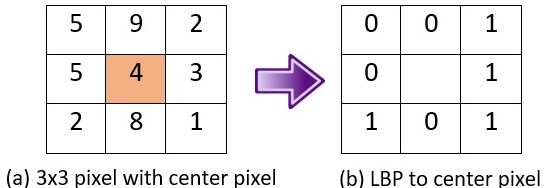
\includegraphics[width=0.6\linewidth]{pic/fig2}
	\caption{LBP Operator.}
	\label{fig:LBP}
\end{figure}
\vspace{1 cm}
\begin{figure}[h!]
	\centering
	\includegraphics[width=0.5\linewidth]{pic/fig3}
	\caption{Example of CLBP Operations.}
	\label{fig:CLBP}
\end{figure}
\vspace{1 cm}
\begin{figure}[h!]
	\centering
	\includegraphics[width=0.99\linewidth]{pic/fig4}
	\caption{Implementation of RLBP.}
	\label{fig:RLBP}
\end{figure}
\vspace{1 cm}

\begin{figure}[h]
	\centering
	\includegraphics[width=0.67\linewidth]{pic/fig5}
	\caption{The implementation of LBP-HF feature for rotation invariant image description.}
	\label{fig:LBP-HF}
\end{figure}
\vspace{1 cm}
\begin{figure}[h!]
	\centering
	\includegraphics[width=0.99\linewidth]{pic/fig6}
	\caption{The concept of LCP.}
	\label{fig:LCP}
\end{figure} 
\vspace{1 cm}
\begin{figure}[h]
	\centering
	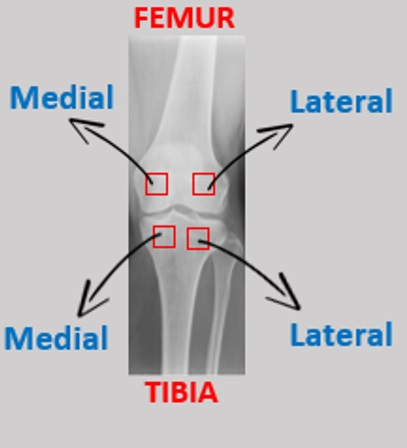
\includegraphics[width=0.5\linewidth]{pic/fig9}
	\caption{The Four ROI of Texture Analysis}
	\label{fig:fig9}
\end{figure}
\end{document}